% Computational cost: main-text subsection, scope sentences and limitation (#181).
% Numbers: artifacts/issue-181/encoded_input_size.md (tokenizer only) and
% artifacts/issue-181/cost_D1.{md,tex} (scripts/encode_timing.py, one
% controlled run on D1 at bf8d7f6; records in artifacts/issue-181/timing/).
% Requires \usepackage{threeparttable} (Table tab:cost_d1) and graphicx (Figure fig:cost_d1).

% --- Scope sentence (introduction, after the contributions list) -----------
% This study measures effectiveness: how embedding model and entity
% verbalisation change the re-ranking of a fixed candidate set. We report
% what each condition costs to compute (Section~\ref{sec:cost}) so that its
% gains can be weighed against it, but we make no efficiency or scalability
% claim.

\subsection{Computational cost}
\label{sec:cost}

This study is about effectiveness, and we make no efficiency claim. A gain in
re-ranking quality is only useful, however, if its cost is known, so we report
what each condition computes and, on the largest biomedical column, how long it
takes.

\paragraph{Cost structure.}
Stage~1 scores every source against all target entities of its type through a
character n-gram index and keeps 20 candidates; it is the same for every
condition and is B0's entire cost. Stage~2 verbalises and encodes every source
and every distinct candidate once, then computes at most 20 cosine
similarities per source. Its cost therefore grows linearly with the number of
entities encoded, and the size of the target graph enters only through stage~1
and the number of distinct candidates. Per text, encoding cost grows with the
text's length, up to the model's token limit, and with model size. The
conditions thus differ in two factors: how much text the verbalisation
produces, and which model encodes it.

\paragraph{Input size.}
Token counts under each model's own tokenizer do not depend on hardware
(\texttt{encoded\_input\_size.md}). Every condition on a column encodes the
same entities (74,285 on D1, 194,547 on D4$_{\mathrm{in}}$, 28,418 on D5), so
the verbalisation decides how much text is encoded. On D1, labels alone (V1) amount
to 1.2M tokens, V2+V8 to 2.7M and key--value context (V3: 8.0M; V6+V3: 12.1M)
to up to ten times as many. On D4$_{\mathrm{in}}$ the spread is 2.3M (V1) to
47.4M (V5), a factor of 21. Key--value texts on the instance columns also
often exceed the model's 512-token limit, because their budget is enforced
on an estimate (1.3 tokens per word) rather than on the tokenizer's count.
The model then truncates them: 14--28\% of the texts encoded by C3, C4, C5
and C7 on D4$_{\mathrm{in}}$, and 24\% under C7 on D5. M4 (BioLORD) truncates
at its own limit of 128 tokens, which cuts 13--22\% of the texts of C6 and
C16 on D1 and D2 but almost none of C11 or C17. Apart from M4, at most 83
texts on D1 exceed the limit in any condition.

\paragraph{Wall-clock cost on D1.}
Table~\ref{tab:cost_d1} times every condition registered on D1 in one
controlled run (an Apple M4 Pro with 64\,GB, PyTorch 2.11 on the MPS backend,
three encoding passes after a warm-up, nothing else running); each run
reproduced its stored metrics exactly, and Figure~\ref{fig:cost_d1} sets each
condition's time against its MRR. Stage~1 takes 22\,s for D1's 24,182
sources. Stage~2 takes from 40\,s (C1, V1/M1) to 54\,min (C13, V2+V8/M5), a
factor of 82. With the text fixed to V2+V8, the model sets the cost: 44\,s
under M1, 4.0\,min under M4, 12.0 under M2, 12.6 under M3 and 54.2 under M5,
for MRR 0.648, 0.687, 0.649, 0.695 and 0.713, so M5 takes 13.7 times as long
as M4 for 0.026 more MRR. With the model fixed to M2, the verbalisation does:
V2 takes 11.3\,min (MRR 0.621), V2+V6 22.4, V3 30.8 (0.779) and V6+V3 44.8,
four times V2, for an MRR (0.710) no better than B0's. The five conditions
significantly above B0 on D1 cost 3.7\,min (C17, V1/M4), 6.8 (C6), 7.2 (C16),
22.4 (C3) and 30.8 (C4); the best of them, C4, takes 8.3 times as long as
C17 for 0.021 more MRR. Token counts predict time only once texts are long:
under M2, V8 (1.3M tokens) takes 11.0\,min and V2+V8 (2.7M) 12.0, while V3
(8.0M) takes 30.8. M4's times are for texts cut at 128 tokens.

These timings describe one implementation on one machine: encoding runs on
Apple's MPS backend and pads every batch to a multiple of 64 tokens, so short
texts cost about the same per batch whatever their length, and it encodes a
condition's texts in smaller batches when their estimated average length is
long. They support comparisons between conditions, not absolute
throughput claims, and they are not comparable with the runtimes of published
systems, which solve a different task (Section~\ref{sec:comparability}).

\begin{table}[t]
\centering
\footnotesize
\setlength{\tabcolsep}{4pt}
\begin{threeparttable}
\caption{Computational cost of stage~2 on D1, one run per condition. Params: model parameters, in millions. Tokens: total encoded tokens, in millions (sources and unique candidates, each capped at the model's limit). Min.: verbalisation, encoding (median of 3 passes) and ranking, in minutes; $\times$: relative to the cheapest condition. Stage~1, shared by every condition and B0's whole cost, takes 22\,s.}
\label{tab:cost_d1}
\begin{tabular}{lllrrrrrr}
\hline
\textbf{Cond.} & \textbf{Text} & \textbf{Model} & \textbf{Params} & \textbf{Tokens} & \textbf{Min.} & $\times$ & \textbf{MRR} & $\Delta$\textbf{B0} \\
\hline
B0 & -- & -- & -- & -- & -- & -- & 0.705 & -- \\
C1 & V1 & M1 & 23 & 1.21 & 0.7 & 1.0 & 0.719 & +0.013 \\
C2 & V2 & M1 & 23 & 1.55 & 0.7 & 1.0 & 0.684 & $-$0.022 \\
C17 & V1 & M4 & 109 & 1.21 & 3.7 & 5.6 & 0.758 & +0.052 \\
C3 & V2+V6 & M2 & 335 & 5.67 & 22.4 & 33.9 & 0.768 & +0.062 \\
C9 & V8 & M2 & 335 & 1.32 & 11.0 & 16.6 & 0.181 & $-$0.525 \\
C10 & V2+V8 & M2 & 335 & 2.72 & 12.0 & 18.1 & 0.649 & $-$0.056 \\
C18 & V2+V8 & M1 & 23 & 2.72 & 0.7 & 1.1 & 0.648 & $-$0.058 \\
C4 & V3 & M2 & 335 & 7.98 & 30.8 & 46.6 & 0.779 & +0.074 \\
C6 & V2+V7 & M4 & 109 & 5.92 & 6.8 & 10.3 & 0.755 & +0.049 \\
C7 & V6+V3 & M2 & 335 & 12.10 & 44.8 & 67.8 & 0.710 & +0.005 \\
C11 & V2+V8 & M4 & 109 & 2.72 & 4.0 & 6.0 & 0.687 & $-$0.018 \\
C13 & V2+V8 & M5 & 1{,}545 & 2.88 & 54.2 & 82.0 & 0.713 & +0.008 \\
C16 & V2+V8+V7 & M4 & 109 & 6.88 & 7.2 & 10.9 & 0.728 & +0.022 \\
C15 & V2+V8 & M3 & 568 & 3.18 & 12.6 & 19.0 & 0.695 & $-$0.011 \\
C20 & V2 & M2 & 335 & 1.55 & 11.3 & 17.1 & 0.621 & $-$0.084 \\
\hline
\end{tabular}
\begin{tablenotes}\footnotesize
\item Timings: Apple M4 Pro, 64 GB, device mps, torch 2.11.0, commit bf8d7f6, 3 timed encoding passes after a warm-up; descriptive, specific to this machine and implementation.
\end{tablenotes}
\end{threeparttable}
\end{table}
  % generated by scripts/generate_cost_report.py

\begin{figure}[t]
\centering
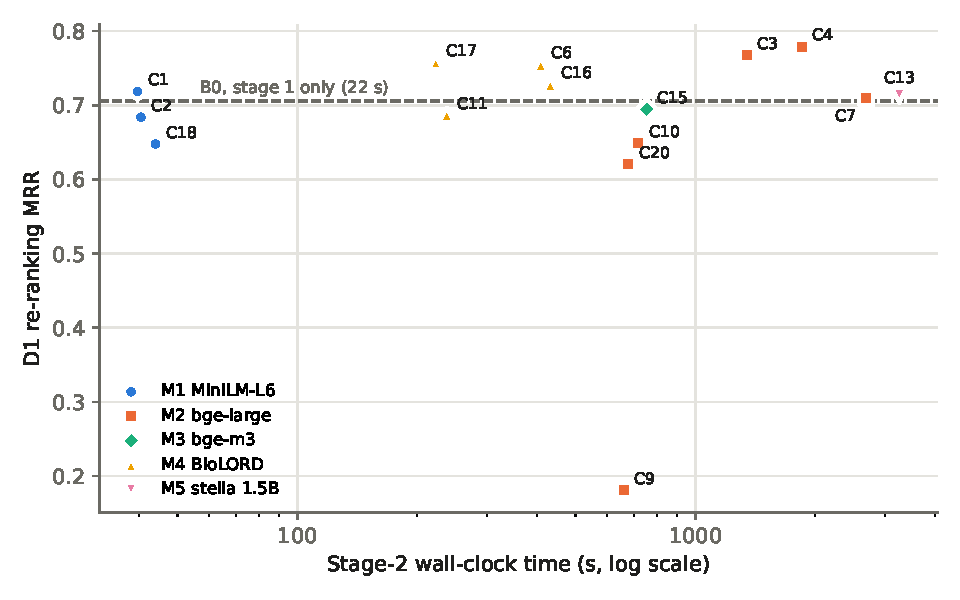
\includegraphics[width=\columnwidth]{cost_vs_mrr_D1.pdf}
\caption{D1 re-ranking MRR against stage-2 wall-clock time (log scale), one
point per condition, coloured by model. The dashed line is B0, which needs
stage~1 only; every condition runs stage~1 as well. Timings as in
Table~\ref{tab:cost_d1}.}
\label{fig:cost_d1}
\end{figure}

% --- Limitation (limitations section) --------------------------------------
% We did not study scalability. Stage~2's cost is linear in the number of
% entities encoded, and the target graph enters it only through stage~1 and
% the number of distinct candidates; stage~1's scaling is outside this paper; the timings of Section~\ref{sec:cost} come
% from one machine and one implementation, and memory use, larger graphs and
% other hardware were not measured.
